% Grafos da aula de representação e percursos. Compartilhado entre o roteiro
% (figuras.tex) e os slides (grafos.tex da pasta 00_grafos). Os grafos são os
% mesmos dos programas da pasta codes.

\tikzset{
  gv/.style = {circle, draw=black, fill=white, inner sep=0pt,
    minimum size=1.6em, line width=0.6pt, font=\sffamily\small},
  ga/.style = {draw=black!55, line width=0.7pt},
  garv/.style = {draw=blue!70!black, line width=2.2pt},
  gnota/.style = {font=\sffamily\scriptsize, text=blue!70!black},
  arco/.style = {-{Stealth[length=2.4mm]}, draw=black!70, line width=0.7pt},
  pv/.style = {rectangle, rounded corners=2pt, draw=black, fill=white,
    inner sep=3pt, line width=0.6pt, font=\ttfamily\small},
  arcov/.style = {-{Stealth[length=2.4mm]}, draw=red!75!black, line width=1.6pt}
}

% ------------------------------------------------------------------
% Grafo G, de bfs.go, dfs.go e representacao.go.
\newcommand{\Gnos}{%
  \node [gv] (g0) at (0, 1.5) {0};
  \node [gv] (g1) at (1.5, 3) {1};
  \node [gv] (g2) at (1.5, 1.5) {2};
  \node [gv] (g5) at (1.5, 0) {5};
  \node [gv] (g3) at (3, 3) {3};
  \node [gv] (g4) at (3, 0) {4};
  \node [gv] (g6) at (4.5, 1.5) {6};
  \node [gv] (g7) at (6, 1.5) {7};
}
\newcommand{\Garestas}{%
  \foreach \a/\b in {0/1, 0/2, 0/5, 1/3, 2/3, 2/4, 3/6, 4/5, 4/6, 6/7}
    \draw [ga] (g\a) -- (g\b);
}

\newcommand{\grafoG}{%
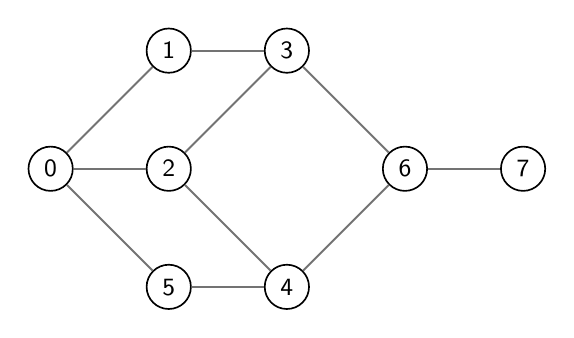
\begin{tikzpicture}
  \Gnos
  \Garestas
\end{tikzpicture}}

% Árvore da busca em largura a partir de 0, com a distância de cada vértice.
\newcommand{\grafoGbfs}{%
\begin{tikzpicture}
  \Gnos
  \Garestas
  \foreach \a/\b in {0/1, 0/2, 0/5, 1/3, 2/4, 3/6, 6/7}
    \draw [garv] (g\a) -- (g\b);
  \Gnos
  \foreach \v/\d/\p in {0/0/left, 1/1/above, 2/1/right, 5/1/below,
                        3/2/above, 4/2/below, 6/3/below, 7/4/above}
    \node [gnota, \p=1pt of g\v] {d=\d};
\end{tikzpicture}}

% Árvore da busca em profundidade a partir de 0, com a ordem de visita.
\newcommand{\grafoGdfs}{%
\begin{tikzpicture}
  \Gnos
  \Garestas
  \foreach \a/\b in {0/1, 1/3, 3/2, 2/4, 4/5, 4/6, 6/7}
    \draw [garv] (g\a) -- (g\b);
  \Gnos
  \foreach \v/\d/\p in {0/1/left, 1/2/above, 3/3/above, 2/4/right,
                        4/5/below, 5/6/below, 6/7/below, 7/8/above}
    \node [gnota, \p=1pt of g\v] {\d\textordmasculine};
\end{tikzpicture}}

% ------------------------------------------------------------------
% Grafo de componentes.go: 10 vértices, 4 componentes.
\newcommand{\grafoComp}{%
\begin{tikzpicture}
  \node [gv] (h0) at (0, 1.6) {0};
  \node [gv] (h1) at (-0.7, 0.4) {1};
  \node [gv] (h2) at (0.7, 0.4) {2};
  \node [gv] (h3) at (2.2, 1.6) {3};
  \node [gv] (h4) at (2.2, 0.4) {4};
  \node [gv] (h5) at (3.7, 1.6) {5};
  \node [gv] (h6) at (5.0, 1.6) {6};
  \node [gv] (h7) at (3.7, 0.4) {7};
  \node [gv] (h8) at (5.0, 0.4) {8};
  \node [gv] (h9) at (6.5, 1.0) {9};
  \foreach \a/\b in {0/1, 0/2, 1/2, 3/4, 5/6, 5/7, 6/8, 7/8}
    \draw [ga] (h\a) -- (h\b);
  \node [gnota, below=0.25cm of h1, xshift=0.7cm] {id 0};
  \node [gnota, below=0.25cm of h4] {id 1};
  \node [gnota, below=0.25cm of h7, xshift=0.65cm] {id 2};
  \node [gnota, below=0.85cm of h9] {id 3};
\end{tikzpicture}}

% ------------------------------------------------------------------
% Pacotes de topologica.go. O arco B -> A significa que A importa B.
\newcommand{\Pnos}{%
  \node [pv] (modelo) at (0, 2.4) {modelo};
  \node [pv] (log) at (0, 1.2) {log};
  \node [pv] (config) at (0, 0) {config};
  \node [pv] (banco) at (2.6, 1.2) {banco};
  \node [pv] (servico) at (5.2, 2.4) {servico};
  \node [pv] (http) at (7.8, 1.2) {http};
  \node [pv] (main) at (10.4, 1.2) {main};
}
\newcommand{\Parcos}{%
  \draw [arco] (modelo) -- (banco);
  \draw [arco] (log) -- (banco);
  \draw [arco] (config) -- (banco);
  \draw [arco] (banco) -- (servico);
  \draw [arco] (modelo) -- (servico);
  \draw [arco] (log) -- (servico);
  \draw [arco] (log) to [bend right=14] (http);
  \draw [arco] (servico) -- (http);
  \draw [arco] (servico) -- (main);
  \draw [arco] (http) -- (main);
  \draw [arco] (config) to [bend right=8] (main);
}
\newcommand{\grafoPacotes}{%
\begin{tikzpicture}
  \Pnos
  \Parcos
\end{tikzpicture}}

% O mesmo grafo com o arco servico -> modelo, que fecha um ciclo.
\newcommand{\grafoPacotesCiclo}{%
\begin{tikzpicture}
  \Pnos
  \Parcos
  \draw [arcov] (modelo) -- (banco);
  \draw [arcov] (banco) -- (servico);
  \draw [arcov] (servico) to [bend right=25] (modelo);
\end{tikzpicture}}

% A ordem topológica encontrada, da esquerda para a direita: todo arco aponta
% para a direita.
\newcommand{\grafoPacotesOrdem}{%
\begin{tikzpicture}
  \foreach \n/\x in {log/0, config/1.7, modelo/3.4, banco/5.1,
                     servico/6.8, http/8.5, main/10.2}
    \node [pv] (\n) at (\x, 0) {\n};
  \draw [arco] (modelo) -- (banco);
  \draw [arco] (banco) -- (servico);
  \draw [arco] (servico) -- (http);
  \draw [arco] (http) -- (main);
  \draw [arco] (log.north) .. controls +(0, 1.0) and +(0, 1.0) .. (banco.north);
  \draw [arco] (log.north) .. controls +(0, 1.4) and +(0, 1.4) .. (servico.north);
  \draw [arco] (log.north) .. controls +(0, 1.8) and +(0, 1.8) .. (http.north);
  \draw [arco] (servico.north) .. controls +(0, 0.8) and +(0, 0.8) .. (main.north);
  \draw [arco] (config.south) .. controls +(0, -0.8) and +(0, -0.8) .. (banco.south);
  \draw [arco] (modelo.south) .. controls +(0, -1.1) and +(0, -1.1) .. (servico.south);
  \draw [arco] (config.south) .. controls +(0, -1.6) and +(0, -1.6) .. (main.south);
\end{tikzpicture}}

% ------------------------------------------------------------------
% Componentes fortemente conexas: três componentes, destacadas pelo fundo.
\newcommand{\grafoCFC}{%
\begin{tikzpicture}
  \fill [orange!18, rounded corners=8pt] (-0.55, -0.6) rectangle (2.05, 2.1);
  \fill [green!18, rounded corners=8pt] (3.15, -0.6) rectangle (5.75, 2.1);
  \fill [blue!12, rounded corners=8pt] (6.85, 0.15) rectangle (7.95, 1.35);
  \node [gv] (c0) at (0, 1.5) {0};
  \node [gv] (c1) at (1.5, 1.5) {1};
  \node [gv] (c2) at (0.75, 0) {2};
  \node [gv] (c3) at (3.7, 1.5) {3};
  \node [gv] (c4) at (5.2, 1.5) {4};
  \node [gv] (c5) at (4.45, 0) {5};
  \node [gv] (c6) at (7.4, 0.75) {6};
  \draw [arco] (c0) -- (c1);
  \draw [arco] (c1) -- (c2);
  \draw [arco] (c2) -- (c0);
  \draw [arco] (c3) -- (c4);
  \draw [arco] (c4) -- (c5);
  \draw [arco] (c5) -- (c3);
  \draw [arco] (c1) -- (c3);
  \draw [arco] (c2) -- (c5);
  \draw [arco] (c4) -- (c6);
\end{tikzpicture}}

% ------------------------------------------------------------------
% Execução passo a passo das duas buscas em G, a partir de 0. Os estados
% seguem a saída de bfs.go e dfs.go. Cores: branco, ainda não alcançado;
% cinza, na fila (largura) ou com a chamada em andamento (profundidade); preto,
% já retirado da fila ou com a chamada terminada. A borda vermelha marca o
% vértice em processamento. Em azul, as arestas da árvore; em laranja, as
% arestas que entraram na árvore no passo.
\tikzset{
  gcinza/.style = {fill=black!25},
  gpreto/.style = {fill=black!80, text=white},
  gatual/.style = {draw=red!80!black, line width=2pt},
  gnova/.style = {draw=orange!90!black, line width=2.6pt},
  gcaixa/.style = {rectangle, draw=black, fill=black!25, line width=0.6pt,
    minimum width=0.55cm, minimum height=0.5cm, inner sep=0pt,
    font=\sffamily\small},
  gquadro/.style = {rectangle, draw=black, fill=black!25, line width=0.6pt,
    minimum width=1.7cm, minimum height=0.36cm, inner sep=0pt,
    font=\ttfamily\scriptsize},
  gtexto/.style = {anchor=west, font=\sffamily\footnotesize, inner sep=0pt},
  gtabela/.style = {anchor=east, font=\ttfamily\small, inner sep=0pt},
  glegenda/.style = {anchor=west, font=\sffamily\scriptsize, inner sep=0pt}
}

% Posição do rótulo de distância em volta de cada vértice, em graus.
\newcommand{\Gang}[1]{\ifcase#1 180\or 90\or 0\or 90\or 270\or 270\or 270\or 90\fi}

% Grafo G no estado de um passo. #1: vértice em processamento (pode ser
% vazio); #2: vértices cinza; #3: vértices pretos; #4: arestas da árvore;
% #5: arestas novas no passo.
\newcommand{\Gestado}[5]{%
  \Gnos
  \Garestas
  \foreach \a/\b in {#4} \draw [garv] (g\a) -- (g\b);
  \foreach \a/\b in {#5} \draw [gnova] (g\a) -- (g\b);
  \Gnos
  \foreach \v in {#2} \node [gv, gcinza] at (g\v) {\v};
  \foreach \v in {#3} \node [gv, gpreto] at (g\v) {\v};
  \foreach \v in {#1} \draw [gatual] (g\v) circle (0.8em);
}

% Um passo da busca em largura. #1 a #5 como em \Gestado; #6: fila, do início
% para o fim; #7: distâncias conhecidas, em pares v/d; #8: o que o passo faz.
\newcommand{\passoBFS}[8]{%
\begin{tikzpicture}
  \useasboundingbox (-1.1, -2.55) rectangle (8.8, 3.65);
  \Gestado{#1}{#2}{#3}{#4}{#5}
  \foreach \v/\d in {#7} {
    \edef\ang{\Gang{\v}}
    \path (g\v) ++(\ang:0.66 and 0.43) node [gnota] {d=\d};
  }
  \node [gtabela] at (7.0, 3.4) {v};
  \node [gtabela] at (7.95, 3.4) {dist};
  \node [gtabela] at (8.75, 3.4) {pai};
  \draw [black!60] (6.6, 3.18) -- (8.8, 3.18);
  \foreach \v in {0, ..., 7}
    \node [gtabela] at (7.0, 2.92 - 0.38*\v) {\v};
  \foreach \v/\d in {#7}
    \node [gtabela] at (7.95, 2.92 - 0.38*\v) {\d};
  \node [gtabela] at (8.75, 2.92) {-1};
  \foreach \a/\b in {#4} \node [gtabela] at (8.75, 2.92 - 0.38*\b) {\a};
  \foreach \a/\b in {#5} \node [gtabela] at (8.75, 2.92 - 0.38*\b) {\a};
  \node [gtexto] at (-1.1, -1.05) {fila:};
  \foreach \v [count=\i] in {#6}
    \node [gcaixa] at (-0.2 + 0.6*\i, -1.05) {\v};
  \node [gtexto] at (-1.1, -1.75) {#8};
  \node [gv, gcinza, minimum size=1em] at (-0.9, -2.35) {};
  \node [glegenda] at (-0.65, -2.35) {na fila};
  \node [gv, gpreto, minimum size=1em] at (0.9, -2.35) {};
  \node [glegenda] at (1.15, -2.35) {já retirado};
  \node [gv, gatual, minimum size=1em] at (3.2, -2.35) {};
  \node [glegenda] at (3.45, -2.35) {retirado agora};
\end{tikzpicture}}

% Um passo da busca em profundidade. #1 a #5 como em \Gestado, com #2 também
% sendo a pilha de chamadas, da base para o topo; #6: pré-ordem até o passo;
% #7: pós-ordem até o passo; #8: o que o passo faz.
\newcommand{\passoDFS}[8]{%
\begin{tikzpicture}
  \useasboundingbox (-1.1, -2.55) rectangle (8.8, 3.65);
  \Gestado{#1}{#2}{#3}{#4}{#5}
  \gdef\Gtopo{0}
  \foreach \v [count=\i] in {#2} {
    \node [gquadro] at (7.9, -0.2 + 0.42*\i) {visita(\v)};
    \xdef\Gtopo{\i}
  }
  \ifnum\Gtopo>0
    \node [gquadro, gatual, fill=none] at (7.9, -0.2 + 0.42*\Gtopo) {};
  \fi
  \node [glegenda, anchor=center] at (7.9, -0.25) {pilha de chamadas};
  \node [gtexto] at (-1.1, -0.85) {pré-ordem: \texttt{#6}};
  \node [gtexto] at (-1.1, -1.3) {pós-ordem: \texttt{#7}};
  \node [gtexto] at (-1.1, -1.75) {#8};
  \node [gv, gcinza, minimum size=1em] at (-0.9, -2.35) {};
  \node [glegenda] at (-0.65, -2.35) {chamada em andamento};
  \node [gv, gpreto, minimum size=1em] at (3.0, -2.35) {};
  \node [glegenda] at (3.25, -2.35) {chamada terminada};
  \node [gv, gatual, minimum size=1em] at (6.4, -2.35) {};
  \node [glegenda] at (6.65, -2.35) {em execução};
\end{tikzpicture}}

% Passos numerados a partir de 1, para \only nos slides.
\newcommand{\bfsPasso}[1]{\ifcase#1
\or\passoBFS{}{0}{}{}{}{0}{0/0}{início: marca o 0 e o põe na fila}
\or\passoBFS{0}{1, 2, 5}{}{}{0/1, 0/2, 0/5}{1, 2, 5}{0/0, 1/1, 2/1, 5/1}{retira 0, lista \texttt{[1 2 5]}: 1, 2 e 5 entram na fila}
\or\passoBFS{1}{2, 5, 3}{0}{0/1, 0/2, 0/5}{1/3}{2, 5, 3}{0/0, 1/1, 2/1, 3/2, 5/1}{retira 1, lista \texttt{[0 3]}: 3 entra na fila}
\or\passoBFS{2}{5, 3, 4}{0, 1}{0/1, 0/2, 0/5, 1/3}{2/4}{5, 3, 4}{0/0, 1/1, 2/1, 3/2, 4/2, 5/1}{retira 2, lista \texttt{[0 3 4]}: 4 entra na fila}
\or\passoBFS{5}{3, 4}{0, 1, 2}{0/1, 0/2, 0/5, 1/3, 2/4}{}{3, 4}{0/0, 1/1, 2/1, 3/2, 4/2, 5/1}{retira 5, lista \texttt{[0 4]}: todos marcados, nada entra}
\or\passoBFS{3}{4, 6}{0, 1, 2, 5}{0/1, 0/2, 0/5, 1/3, 2/4}{3/6}{4, 6}{0/0, 1/1, 2/1, 3/2, 4/2, 5/1, 6/3}{retira 3, lista \texttt{[1 2 6]}: 6 entra na fila}
\or\passoBFS{4}{6}{0, 1, 2, 5, 3}{0/1, 0/2, 0/5, 1/3, 2/4, 3/6}{}{6}{0/0, 1/1, 2/1, 3/2, 4/2, 5/1, 6/3}{retira 4, lista \texttt{[2 5 6]}: todos marcados, nada entra}
\or\passoBFS{6}{7}{0, 1, 2, 5, 3, 4}{0/1, 0/2, 0/5, 1/3, 2/4, 3/6}{6/7}{7}{0/0, 1/1, 2/1, 3/2, 4/2, 5/1, 6/3, 7/4}{retira 6, lista \texttt{[3 4 7]}: 7 entra na fila}
\or\passoBFS{7}{}{0, 1, 2, 5, 3, 4, 6}{0/1, 0/2, 0/5, 1/3, 2/4, 3/6, 6/7}{}{}{0/0, 1/1, 2/1, 3/2, 4/2, 5/1, 6/3, 7/4}{retira 7, lista \texttt{[6]}: fila vazia, fim da busca}
\fi}
\newcommand{\dfsPasso}[1]{\ifcase#1
\or\passoDFS{0}{0}{}{}{}{0}{}{\texttt{visita(0)}: lista \texttt{[1 2 5]}, desce para o 1}
\or\passoDFS{1}{0, 1}{}{}{0/1}{0 1}{}{\texttt{visita(1)}: lista \texttt{[0 3]}, 0 já marcado, desce para o 3}
\or\passoDFS{3}{0, 1, 3}{}{0/1}{1/3}{0 1 3}{}{\texttt{visita(3)}: lista \texttt{[1 2 6]}, 1 já marcado, desce para o 2}
\or\passoDFS{2}{0, 1, 3, 2}{}{0/1, 1/3}{3/2}{0 1 3 2}{}{\texttt{visita(2)}: lista \texttt{[0 3 4]}, 0 e 3 já marcados, desce para o 4}
\or\passoDFS{4}{0, 1, 3, 2, 4}{}{0/1, 1/3, 3/2}{2/4}{0 1 3 2 4}{}{\texttt{visita(4)}: lista \texttt{[2 5 6]}, 2 já marcado, desce para o 5}
\or\passoDFS{5}{0, 1, 3, 2, 4, 5}{}{0/1, 1/3, 3/2, 2/4}{4/5}{0 1 3 2 4 5}{}{\texttt{visita(5)}: lista \texttt{[0 4]}, todos marcados}
\or\passoDFS{4}{0, 1, 3, 2, 4}{5}{0/1, 1/3, 3/2, 2/4, 4/5}{}{0 1 3 2 4 5}{5}{\texttt{termina 5}: volta ao 4; o 6 não está marcado}
\or\passoDFS{6}{0, 1, 3, 2, 4, 6}{5}{0/1, 1/3, 3/2, 2/4, 4/5}{4/6}{0 1 3 2 4 5 6}{5}{\texttt{visita(6)}: lista \texttt{[3 4 7]}, 3 e 4 já marcados, desce para o 7}
\or\passoDFS{7}{0, 1, 3, 2, 4, 6, 7}{5}{0/1, 1/3, 3/2, 2/4, 4/5, 4/6}{6/7}{0 1 3 2 4 5 6 7}{5}{\texttt{visita(7)}: lista \texttt{[6]}, todos marcados}
\or\passoDFS{6}{0, 1, 3, 2, 4, 6}{5, 7}{0/1, 1/3, 3/2, 2/4, 4/5, 4/6, 6/7}{}{0 1 3 2 4 5 6 7}{5 7}{\texttt{termina 7}: volta ao 6; fim da lista}
\or\passoDFS{4}{0, 1, 3, 2, 4}{5, 7, 6}{0/1, 1/3, 3/2, 2/4, 4/5, 4/6, 6/7}{}{0 1 3 2 4 5 6 7}{5 7 6}{\texttt{termina 6}: volta ao 4; fim da lista}
\or\passoDFS{2}{0, 1, 3, 2}{5, 7, 6, 4}{0/1, 1/3, 3/2, 2/4, 4/5, 4/6, 6/7}{}{0 1 3 2 4 5 6 7}{5 7 6 4}{\texttt{termina 4}: volta ao 2; fim da lista}
\or\passoDFS{3}{0, 1, 3}{5, 7, 6, 4, 2}{0/1, 1/3, 3/2, 2/4, 4/5, 4/6, 6/7}{}{0 1 3 2 4 5 6 7}{5 7 6 4 2}{\texttt{termina 2}: volta ao 3; 6 já marcado, fim da lista}
\or\passoDFS{1}{0, 1}{5, 7, 6, 4, 2, 3}{0/1, 1/3, 3/2, 2/4, 4/5, 4/6, 6/7}{}{0 1 3 2 4 5 6 7}{5 7 6 4 2 3}{\texttt{termina 3}: volta ao 1; fim da lista}
\or\passoDFS{0}{0}{5, 7, 6, 4, 2, 3, 1}{0/1, 1/3, 3/2, 2/4, 4/5, 4/6, 6/7}{}{0 1 3 2 4 5 6 7}{5 7 6 4 2 3 1}{\texttt{termina 1}: volta ao 0; 2 e 5 já marcados, fim da lista}
\or\passoDFS{}{}{5, 7, 6, 4, 2, 3, 1, 0}{0/1, 1/3, 3/2, 2/4, 4/5, 4/6, 6/7}{}{0 1 3 2 4 5 6 7}{5 7 6 4 2 3 1 0}{\texttt{termina 0}: fim da busca}
\fi}

% ------------------------------------------------------------------
% Balde de tinta: imagem de 10 por 7 pixels, com 4 vizinhos por pixel. #1 = 0
% mostra a imagem antes do clique; #1 = 1, depois, com a componente do pixel
% clicado pintada.
\newcommand{\imagemBalde}[1]{%
\begin{tikzpicture}[x=0.38cm, y=0.38cm]
  \foreach \x/\y in {2/2, 3/2, 4/2, 5/2, 6/2, 7/2, 2/3, 3/3, 6/3, 7/3, 2/4, 3/4, 4/4, 5/4, 6/4, 7/4}
    {\ifnum#1=1 \fill [orange!70] (\x, -\y) rectangle ++(1, -1);\fi}
  \foreach \x/\y in {2/1, 3/1, 4/1, 5/1, 6/1, 7/1, 1/2, 8/2, 1/3, 4/3, 5/3, 8/3, 1/4, 8/4, 2/5, 3/5, 4/5, 5/5, 6/5, 7/5}
    \fill [black!80] (\x, -\y) rectangle ++(1, -1);
  \draw [black!25, line width=0.3pt] (0, 0) grid (10, -7);
  \draw [black, line width=0.6pt] (0, 0) rectangle (10, -7);
  \fill [red!80!black] (2.5, -3.5) circle (0.18);
  \node [font=\sffamily\scriptsize, anchor=north] at (5, -7.2)
    {\ifnum#1=1 depois do clique\else antes do clique\fi};
\end{tikzpicture}}

% ------------------------------------------------------------------
% Memória de um programa: objetos e ponteiros. Os objetos que as raízes não
% alcançam são lixo.
\newcommand{\grafoMemoria}{%
\begin{tikzpicture}
  \node [pv, font=\sffamily\small] (raiz) at (0, 1.2) {raízes};
  \node [gv] (a) at (2, 2) {a};
  \node [gv] (b) at (2, 0.4) {b};
  \node [gv] (c) at (3.6, 2) {c};
  \node [gv] (d) at (3.6, 0.4) {d};
  \node [gv, gcinza, dashed] (e) at (5.6, 2) {e};
  \node [gv, gcinza, dashed] (f) at (5.6, 0.4) {f};
  \node [gv, gcinza, dashed] (g) at (7.0, 1.2) {g};
  \draw [arco] (raiz) -- (a);
  \draw [arco] (raiz) -- (b);
  \draw [arco] (a) -- (c);
  \draw [arco] (b) -- (d);
  \draw [arco] (d) -- (c);
  \draw [arco] (e) -- (f);
  \draw [arco] (f) -- (g);
  \draw [arco] (e) -- (c);
  \node [gnota, text=black!60, above=0.1cm of e, xshift=0.7cm] {lixo};
\end{tikzpicture}}
